% Preamble -----------------------------------------------------------------------------
    \documentclass[12pt]{article}
% Packages
    \usepackage[utf8]{inputenc}
    \usepackage{xcolor}
    \usepackage{amsmath,amsfonts,amssymb}
    \usepackage[english,spanish]{babel}
    \usepackage[left=2.00cm, right=2.00cm, top=2.00cm, bottom=2.00cm]{geometry}
    \usepackage{float}
    \usepackage{graphicx, graphics}
    \usepackage{hyperref}
    \linespread{1.5}
    \usepackage{multicol}
    \usepackage{url}
    \usepackage{caption}
    \usepackage{subcaption}
    \captionsetup[table]{
       name = Tabla,
       labelsep = newline,
       justification = raggedright,
       singlelinecheck = false,
       labelfont = bf,
    }
    \usepackage{booktabs}
    \usepackage{multirow}
    \usepackage{tabularx}
% Document ----------------------------------------------------------------------------
\begin{document}
    % Resumen
    \begin{flushleft}
        \vspace{6cm}
        {\huge \textbf{Determinantes de la supervivencia empresarial de las mypes peruanas ante eventos como la crisis sanitaria}}\\
        \vspace{2mm}
        { \Large
            Wilder Santos \footnote{Universidad Nacional del Callao},
            Jhon Roly Ordoñez \footnote{Universidad Nacional de San Cristóbal de Huamanga},
            Luis Mendiola \footnote{Universidad Nacional Mayor de San Marcos}
        }
    \end{flushleft}
    % Abstract
    \begin{otherlanguage}{spanish}
        \begin{abstract}
            El objetivo principal de esta investigación es examinar los factores internos de las mypes peruanas
            que influyen en la probabilidad de supervivencia ante escenarios como la crisis sanitaria.
            Para el estudio realizamos un análisis de dos etapas: la primera implicó un análisis de asociación
            unidimensional sobre la variable de estado de las empresas encuestadas, las variables explicativas a
            considerar fueron las disponibles en la base de datos, que han sido estudiadas en estudios previos y que
            han seguido una adecuada intuición económica. Luego, se implementó un modelo de tipo logit con el objetivo
            de cuantificar los efectos marginales de cada variable. Los resultados muestran que un incremento del 1\%
            en los años de funcionamiento de una empresa incrementó la probabilidad de seguir operando en situación
            de pandemia en 0.03\%. Asimismo, si las empresas fueron lideradas por una mujer, aumentó la probabilidad
            de seguir vigente en el mercado en 0.4\%; mientras que, si la empresa hubiese pertenecido al sector
            de Servicios de Mercado la probabilidad de supervivencia se redujo en 0.05\%.
            si las empresas accedieron al programa de Reactiva Perú, la probabilidad de seguir operando en el segundo
            trimestre se redujo en 0.05\%; mientras que, si accedió al Subsidios de trabajadores que recibían un sueldo
            no mayor a S/1500, la probabilidad de seguir operando de abril a junio de 2020 se incrementó en 0.06\%.
            Finalmente, la investigación permite concluir que las estimaciones indican que la presencia de la mujer
            como líder de una empresa asegura la supervivencia de la misma, y que a mayor cantidad de años operando
            en el mercado, se puede soportar shocks tan graves como los dejados por la pandemia.\\
            \textbf{Palabras clave:} \hspace{1mm} \textit{Supervivencia, mypes, Crisis Sanitaria}
        \end{abstract}
    \end{otherlanguage}
    \newpage
    \begin{otherlanguage}{english}
        \begin{abstract}
            The main objective of this research is to examine the internal factors of Peruvian mypes that influence
            the probability of survival in scenarios such as the health crisis. For the study, we carried out a
            two-stage analysis: the first involved a one-dimensional association analysis on the status variable of
            the companies surveyed, the explanatory variables to consider were those available in the database,
            which have been studied in previous studies, and who have followed an adequate economic intuition.
            Then, a logit type model was implemented in order to quantify the marginal effects of each variable.
            The results show that a 1\% increase in the years a company has been in operation increased the probability
            of continuing to operate in a pandemic situation by 0.03\%. Likewise, if the companies were led by a woman,
            the probability of remaining in force in the market increased by 0.4\%; while if the company had belonged
            to the Market Services sector, the probability of survival was reduced by 0.05\%. if the companies agreed
            to the Reactiva Peru program, the probability of continuing to operate in the second quarter was reduced
            by 0.05\%; while, if you accessed the Subsidies for workers who received a salary of no more than S/1500,
            the probability of continuing to operate from April to June 2020 increased by 0.06\%. Finally, the research
            allows us to conclude that the estimates indicate that the presence of a woman as a company leader ensures
            its survival, and that the more years it has been operating in the market, it can withstand shocks
            as serious as those caused by the pandemic.\\
            \textbf{Key Words:} \hspace{1mm} \textit{Survival, mypes, Health Crisis}
        \end{abstract}
    \end{otherlanguage}
    \newpage
    %\begin{multicols}{2}
        %% Section 1
        \section{Introducción}
        {\Huge L}a crisis sanitaria puso en evidencia la vulnerabilidad de los sistemas de salud de los países
        del mundo, la capacidad de resiliencia de las economías, y la capacidad de respuesta de los gobernantes
        del mundo para lidiar con una crisis que amenazaba con terminar con los beneficios de la globalización,
        con el cierre de fronteras, la limitación de importaciones, la libre movilización de las personas, etc.
        Todas estas limitaciones tuvieron como consecuencia la desaceleración de varias economías del mundo, y la
        peruana no fue ajena a ello. Como consecuencia de la desaceleración desaparecieron muchos negocios, sobre
        todo pequeños. Aquellos que lograron sobrevivir, de acuerdo a Barry et al. (2022) se caracterizan porque cuentan
        con flexibilidad financiera (acceso a financiamiento), capacidad de adaptarse para trabajar remotamente,
        y capacidad para diferir o adelantar inversiones (en la medida que las pensiones del mercado lo permitan);
        el tener alguna de estas o todas juntas permiten que una empresa pueda adaptarse mejor a cambios bruscos en
        el mercado. Es a partir de estas tres características que nos planteamos qué otras características o factores
        han podido incidir en que las pequeñas y medianas empresas, en el caso peruano, tengan mayores probabilidades
        de sobrevivir a una crisis como la sanitaria. Dado que en el Perú las empresas más afectadas fueron las micro y
        pequeñas empresas (MYPEs), las que al año 2020, representaron más del 95\% del número de empresas en el país,
        emplearon a 26.6\% de la PEA, siendo otros impactos un incremento de la informalidad, pasando de 81\% en 2017
        a 85\% en 2020, y ventas por 61 mil millones de soles en 2020, 59.2\% menos que en 2019. Como resultado de
        esto, muchas de las MYPEs han tenido que reinventarse para poder sobrevivir, y precarizado aún más las
        condiciones de trabajo de sus colaboradores. En ese sentido la presente investigación, constituye un aporte
        para que los hacedores de política comprendan un poco mejor las características de su grupo objetivo, y a partir
        de este diseñar políticas más efectivas que promuevan la viabilidad financiera de las empresas.
        %% Section 2
        \section{Marco teórico}
        De acuerdo con \cite{Chit}, la sobrevivencia de las empresas puede ser vista, al menos desde dos
        perspectivas teóricas del campo de la administración: la de recursos y capacidades \cite{Penrose}, la teoría de sistemas
        de negocios y la teoría de las variedades de capitalismo (ambas variantes de la teoría institucional).
        La teoría de recursos y capacidades, propone que una empresa que posee recursos internos como activos fijos,
        formación del capital humano, nivel de desarrollo tecnológico, talento de la gente, patentes, licencias, etc.
         \cite{Wernerfelt}, los puede combinar junto a sus capacidades organizacionales y competencias de la gerencia
        que las hacen difíciles de imitar por la competencia, valiosos para la organización, raros y difíciles de
        sustituir \cite{Barney}, para generar una ventaja competitiva.
        La teoría de sistemas de negocios de \cite{Whitley} muestra cómo se forjan las interacciones entre empresas
        e instituciones a lo largo del tiempo y cómo éstas dan lugar a un tipo particular de sistema de negocios
        dentro de una sociedad. Por otro lado, las variedades de capitalismo (Aguilera et al. 2016), se refieren a
        las configuraciones dominantes en los países, que son moldeadas por la estructura de propiedad y el desarrollo
        de las instituciones, en ese sentido se pueden reconocer nueve tipos de variedades de capitalismo, desde el
        liderado por las familias, pasando por los grupos tribales, coordinados por el Estado y los completamente
        orientados por el mercado. Países como el Perú, Colombia, Brasil y México son considerados como capitalismos
        donde la familia es quien lidera el proceso económico y de desarrollo institucional.
        %% Section 3
        \section{Revisión de literatura}
        Muchas de la investigación de los efectos de la crisis sanitaria se han realizado sobre pequeñas y medianas
        empresas, pero en países desarrollados, descuidando la investigación en países emergentes (Yue et al. 2021).
        En \cite{Gamboa}, se analizan los factores que influyen en el desarrollo de las pymes durante el covid,
        para lo cual se realizó una exhaustiva revisión de literatura y análisis de encuestas, encontrándose que los
        principales factores que afectan la viabilidad de las empresas son la producción y el poder cubrir los gastos de
        personal como factores externos, y la crisis sanitaria e inestabilidad de mercado como principales factores externos.
        En Wagner (2022), con información de encuestas conducidas en 2019 y 2020 por el  Banco Mundial, en 10 países europeos,
        se analiza la relación entre el género del propietario con la probabilidad de sobrevivencia de las empresas,
        controlado por las características de las empresas; encontrándose una relación positiva entre que si la empresa
        es propiedad de una mujer hay mayores probabilidades de supervivencia, durante situaciones de shock de oferta y
        demanda como en la crisis sanitaria, este resultado puede ser explicado por la aversión al riesgo por género,
        las mujeres suelen asumir menos riesgos que los hombres.
        Bottazzi et al (2010), estudian la relevancia de las variables financieras y económicas de las empresas que
        cotizan en bolsa y empresas que tienen una responsabilidad limitada. Asimismo, realizan pruebas no paramétricas
        que les permita evaluar en qué medida las empresas que incumplen difieren de las que sí cumplen, y mediante
        las regresiones probit bootstrap constatan que efectivamente las variables económicas tienen un efecto en el
        corto y largo plazo. Además, muestran que las características industriales de las unidades económicas como la
        productividad, el tamaño, la rentabilidad y el crecimiento, sí juegan un rol relevante como determinantes de
        la morosidad. Finalmente, señalan que sus hallazgos son sólidos con respecto al espacio de incumplimiento y
        las calificaciones de riesgo.
        Zhang y Fang (2022), investigan si las pymes ecológicas son menos vulnerables durante la pandemia de COVID-19
        que las pymes convencionales y las grandes empresas. Asimismo, realizan un análisis empírico utilizando los
        datos de la Encuesta de Empresas del Banco Mundial y las encuestas de seguimiento sobre las consecuencias
        económicas de COVID-19, centrándose en 14 países miembros de la Unión Europea. Además, realizan la estimación
        de varios modelos logit ordinal que les permite revelar evidencia de que las pymes y las empresas ecológicas
        tienen una menor probabilidad de verse gravemente afectadas por una situación de crisis sanitaria o pandemia, y
        también señalan que sus hallazgos empíricos probablemente puedan ser explicados por el estado financiero saludable
        de las pymes que han sido respetuosas del medio ambiente antes de la pandemia, indicando las unidades económicas
        de muestra son de estados miembros de la Unión Europea con un alto nivel de desarrollo financiero.
        %% Section 4
        \section{Definición de la Metodología}
        El trabajo ha empleado información de la Encuesta de Opinión sobre el impacto del COVID-19 en las empresas
        realizado por el Instituto Nacional de Estadística e Informática (INEI) en julio de 2020. Según su Ficha Técnica,
        uno de los objetivos de la encuesta fue el elaborar indicadores sobre aspectos cualitativos en los temas relacionados
        a las ventas, empleo, finanzas, expectativas y accesos a los programas del gobierno, vinculados a los efectos del COVID-19,
        en las empresas, por lo que se consideró que los datos permitirán responder los planteamientos establecidos en la parte inicial.
    
        La encuesta fue desarrollada a 1600 empresas ubicadas en Lima Metropolitana y Callao; asimismo, se consideraron casi 
        todos los sectores contenidos en la Clasificación Industrial Internacional Uniforme
        (CIIU)\footnote{Los sectores están relacionados a las secciones de la CIIU revisión 4 disponible
        en: \textcolor{blue}{\url{https://www.gob.pe/institucion/sunat/informes-publicaciones/394120-clasificacion-industrial-internacional-uniforme-ciiu }}}

        La estimación del modelo se ha realizado mediante el software Stata. Se empleó un análisis de dos etapas.
        La primera etapa implicó un análisis de asociación unidimensional sobre la variable de estado de las empresas encuestadas,
        las variables explicativas a considerar fueron las disponibles en la base de datos, que han sido revisadas en estudios previos
        y que han seguido una adecuada intuición económica. Luego, se implementó un modelo de tipo logit con el objetivo de
        cuantificar los efectos marginales de cada variable.
        %% Section 5
        \section{Análisis empírico}
        Tal como se mencionó en la sección anterior, la Tabla 1 muestra los resultados estadísticos sobre la asociación
        que tienen las variables explicativas candidatas a ser parte de la especificación del modelo propuesto en el documento.
        Los resultados indican la existencia de variables que, estadísticamente, presentan evidencia de asociación
        con el estado de operatividad de la empresa en el segundo trimestre de 2020. Sin embargo, también
        se han considerado variables que, aunque no han presentado una asociación individual con la dependiente,
        se encuentran sustentadas por la literatura revisada y por la intuición económica que subyace al modelo propuesto.

        Se encontró que los años de funcionamiento de una empresa posee una asociación directa con el hecho de que la empresa
        siga en funcionamiento durante parte del primer año de la pandemia, siendo 14 años de existencia el promedio del grupo
        de empresas que se mantuvieron vigentes. Por otro lado, se halló que las empresas que siguieron operando en el segundo
        trimestre de 2020 presentaron una menor disminución de las ventas con respecto al mismo periodo del año previo.

        Además, la proporción de empresas que continuaron operativas y mantuvieron retrasos en el pago de facturas fue
        mayor que aquellas que dejaron de operar. Con respecto a las medidas laborales, la proporción de empresas que
        se mantuvieron en el mercado fue mayor en aquellas que decidieron flexibilizar los horarios de trabajo y reducir
        las horas trabajadas durante la semana.

        Por otra parte, existe evidencia que el grupo de empresas que siguieron operando en los meses de abril a junio de 2020
        y que presentaron problemas para cobrar a los clientes fue mayor al grupo que pasaron a estar inoperativos.
        Finalmente, fue mayor la proporción de las empresas que accedieron a programas del gobierno como la Suspensión y
        Modificación de pagos por conceptos de IR y a programas como Reactiva que continuaron operativas en el
        segundo trimestre de 2020.
        % Tabla 1
            \begin{table}[H]
                \raggedright
                \caption{Resumen del Análisis Estadístico de las variables seleccionadas para la especificación del modelo}
                \begin{tabular}{m{7.5cm}ccc}
                    \toprule
                    \multirow{2}{*}{Variable} &  \multicolumn{2}{c}{¿Estuvo operativo en el 2T - 2020?}  & \multirow{2}{*}{Significancia} \\
                    \cline{2-3}  & No & Sí & \\
                    \midrule
                    Años de funcionamiento & 10 & 14 & * \\
                    \hline
                     Variación porcentual de Ventas & -82\% & -53\%  & *** \\
                    \hline
                    Si la empresa pertenece al Sector de servicios de mercado  & 82\%  & 78\%  &  \\
                    \hline
                    Si la empresa adoptó alguna forma de ventas no presenciales & 92\% & 75\% &  \\
                    \hline
                    Sexo del tomador de decisiones de la empresa & 54\% & 64\%  &  \\
                    \hline
                    Adoptó la modalidad de trabajo remoto o mixto por el COVID-19 & 68\% & 61\%  &  \\
                    \hline
                    Problemas: Retraso en el pago de facturas & 23\% & 45\%  & ** \\
                    \hline
                    Medidas laborales: Flexibilidad de horarios & 10\% & 53\%  & *** \\
                    \hline
                    Medidas laborales: Reducción de horas trabajadas en la semana & 7\% & 42\%  & *** \\
                    \hline
                    Problemas financieros: Dificultad para cobrar a los clientes & 19\% & 44\%  & *** \\
                    \hline
                    Accedió al Subsidio a la planilla por Decreto de Urgencia (35\%) & 16\% & 26\%  &  \\
                    \hline
                    Determinación de pagos a cuentas del IR (suspender y modificar) & 1\% & 12\% & *** \\
                    \hline
                    Reactiva Perú & 27\% & 45\%  & * \\
                    \bottomrule
                \end{tabular}
                \caption*{\it Nota: Elaboración Propia, * Sig. 10\%, ** Sig. 5\%, *** Sig. 1\%, para las variables categóricas se realizó la prueba de independencia de $\chi^{2}$ de Pearson, mientras que para las variables cuantitativas se realizó la prueba de Wald ajustada. }
                \label{tab: Tabla1}
            \end{table}
        %% Section 6
        \section{Estimación del modelo, resultados e interpretación}
        A partir del paso previo, se planteó un modelo con las mejores características estadísticas y que se adecúe a los objetivos
        de la investigación, se realizaron las pruebas necesarias para especificar el modelo logit que nos llevará a calcular
        los efectos marginales. Debemos considerar que, en esta parte de la estimación, se están considerando la importancia
        relativa y controlada de las relaciones de las variables. Así la ecuación indexada del modelo especificado es:
            \begin{equation}
                EF_{i} = \beta_{0} + \beta_{1}\ln{\left(AF_{i}\right)} + \beta_{2}SR_{i} + \beta_{3}SM_{i} + \beta_{4}MV_{i} + \beta_{5}MT_{i} + \beta_{5}PRP_{i} + \beta_{6}Sub35_{i} + \varepsilon_{i}
            \end{equation}
        Donde:
            \begin{itemize}
                \item Estado de Funcionamiento (EF), Años de Funcionamiento (AF).
                \item Sexo del Responsable (SR): Es el género del tomador de decisiones de la empresa. Para la encuesta se consideró al propietario, al gerente general o administrador del negocio (0 = Hombre, 1 = Mujer).
                \item Servicio de Mercado (SM): Si pertenece al Agregado Económico de Servicios de Mercado como Comercio; Transporte; Alojamiento y alimentación; y Servicios comerciales y administrativos (0 = No, 1 = Si).
                \item Modalidad de Ventas (MV): (0 = Solo presencia, 1 = No presencial o mixta).
                \item Modalidad de Trabajo (MT): (0 = Solo Presencial, 1 = Trabajo remoto o mixto).
                \item Programa Reactiva Perú (PRP): Se refiere a si accedió o no al programa Reactiva Perú (0 = No, 1 = Si).
                \item Subsidio de 35\% por Decreto de Urgencia (Sub35): Se refiere a si accedió o no al Subsidio del 35\% a trabajadores que ganan hasta S/1500 (0 = No, 1 = Si).
            \end{itemize}
        Una vez realizada la estimación del modelo logístico se calculan los efectos marginales, la Tabla 2 indica que,
        un incremento del 1\% en los años de funcionamiento de una empresa incrementó la probabilidad de seguir operando
        en situación de pandemia en 0.03\%. Asimismo, si las empresas fueron lideradas por una mujer, aumentó la probabilidad
        de seguir vigente en el mercado en 0.4\%; mientras que, si la empresa hubiese pertenecido al sector de Servicios
        de Mercado la probabilidad de supervivencia se redujo en 0.05\%.

        Con respecto a las actividades remotas, se calcula que, el realizar las ventas de forma no presencial redujo la probabilidad
        de seguir operando en 0.01\%, lo mismo que en el caso de los trabajos que optaron por una modalidad de trabajo remoto
        o mixta, en esta situación la probabilidad se redujo en 0.09\%.

        Finalmente, si las empresas accedieron al programa de Reactiva Perú, la probabilidad de seguir operando en el segundo
        trimestre se redujo en 0.05\%; mientras que, si accedió al Subsidios de trabajadores que recibían un sueldo no mayor a S/1500,
        la probabilidad de seguir operando de abril a junio de 2020 se incrementó en 0.06\%.
        % Tabla 2
            \begin{table}[H]
                \raggedright
                \caption{Efectos marginales sobre el modelo Logit para calcular probabilidad de operatividad de una empresa en el segundo trimestrede 2020}
                \begin{tabular}{cccc}
                    \toprule
                    \multicolumn{4}{c}{Efectos marginales}\\
                    \midrule
                     & Mín $\longrightarrow$ Máx & 0 $\longrightarrow$ 1 & Efectos Marginales \\
                    \hline
                    $\ln\left(AF\right)$ & 0.0049 & 0.0035 & 0.0003 \\
                    \hline
                    SR & 0.0038 & 0.0038 & 0.0011\\
                    \hline
                    SM & -0.0005 & -0.0005 & -0.0005\\
                    \hline
                    MV & -0.0001 & -0.0001  & -0.0001\\
                    \hline
                    MT & -0.0009 & -0.0009 & -0.0014\\
                    \hline
                    ARP & -0.0005 & -0.0005 & -0.0005\\
                    \hline
                    Sub35 & 0.0006 & 0.0006 & 0.0006\\
                    \bottomrule
                \end{tabular}
                \caption*{\it Nota: Elaboración Propia}
                \label{tab: Tabla2}
            \end{table}
        %% Section 7
        \section{Conclusiones}
        La encuesta de Opinión de las empresas ha revelado información relevante para entender el impacto de shocks
        en la operatividad del sector empresarial de Lima Metropolitana y Callao. Así, se encontró que 1 de cada 4
        empresas que operaban al inicio de la pandemia dejaron de hacerlo para el segundo trimestre de 2020 (Ver Anexo 2).
        Los sectores donde se paralizaron más las empresas fue en la actividad de Actividades Artísticas, Entretenimiento y Recreación.
        Los problemas más frecuentes declarados por las empresas, fueron los relacionados a la disminución de la demanda,
        los altos costos en seguridad en el marco del COVID-19 y la paralización de la producción (Ver Anexo 5).
        Mientras que, con respecto a los problemas de carácter financiero la falta de liquidez para pagar las remuneraciones
        y a los proveedores fueron los más frecuentes según las declaraciones de los empresarios (Ver Anexo 7).

        Asimismo, con respecto a lo laboral, como principales medidas tomadas para paliar los efectos que sufrían por
        el desarrollo de la pandemia, la flexibilidad de horarios para laborar y la reducción de horas de trabajo
        semanal fueron de las más recurrentes (Ver Anexo 6). Por otro lado, un importante grupo de empresas no accedieron
        a los programas del gobierno como Reactiva Perú, el Subsidio de 35\% a los trabajadores que ganaban hasta S/1500
        o la medida de Suspensión Perfecta de Labores (Ver Anexo 9). Y, las empresas que contaban un mayor tiempo en el
        mercado presentaron menos problemas que las obligaron a dejar de operar en el mercado (Ver Anexo 10).

        Asimismo, con respecto a lo laboral, como principales medidas tomadas para paliar los efectos que sufrían por el
        desarrollo de la pandemia, la flexibilidad de horarios para laborar y la reducción de horas de trabajo semanal
        fueron de las más recurrentes (Ver Anexo 6). Por otro lado, un importante grupo de empresas no accedieron a los
        programas del gobierno como Reactiva Perú, el Subsidio de 35\% a los trabajadores que ganaban hasta S/1500 o
        la medida de Suspensión Perfecta de Labores (Ver Anexo 9). Y, las empresas que contaban un mayor tiempo en el
        mercado presentaron menos problemas que las obligaron a dejar de operar en el mercado (Ver Anexo 10).
        %% References
        \newpage
        \bibliographystyle{apa}
        \begin{thebibliography}{10}
            \bibitem{Barney} J. B. Barney, Firm resources and sustained competitive advantage. Journal of Management, 17, 99-120
            \bibitem{Barrero} Barrero, J. M., Bloom, N., Davis, S. J., 2021. Why working from home will stick. Working Paper 28731, National Bureau of Economic Research.
            \bibitem{Bottazzi} Bottazzi, G., Grazzi, M., Secchi, A., \& Tamagni, F. (2011). Financial and economic determinants of firm default. \textit{Journal of Evolutionary Economics}, 21(3), 373-406.
            \bibitem{Chit} Chit, M. M., Croucher, R., \& Rizov, M. (2022). Surviving the COVID‐19 pandemic: The antecedents of success among European SMEs. In European Management Review. Wiley. \textcolor{blue}{\url{https://doi.org/10.1111/emre.12525}}
            \bibitem{ComexPerú} ComexPerú (2020). Las micro y pequeñas empresas en el Perú Resultados en 2020. \textcolor{blue}{\url{https://www.comexperu.org.pe/upload/articles/reportes/reporte-mypes-2020.pdf}}
            \bibitem{Gamboa} Gamboa, D., \& López, R. (2021). Factores del declive empresarial de las pequeñas empresas del municipio de Ocaña en época de la pandemia, Covid 19. Universidad San Francisco de Paula.
            \bibitem{Penrose} Penrose, E. (1959). The Theory of the Growth of the Firm. Oxford: Oxford University Press.
            \bibitem{Wagner} Wagner, J. (2022). Firm Survival and Gender of Firm Owner in Times of COVID-19: Evidence from 10 European Countries. In Economies (Vol. 10, Issue 5, p. 98). MDPI AG. \textcolor{blue}{\url{https://doi.org/10.3390/economies10050098}}
            \bibitem{Wernerfelt} Wernerfelt, B. (1984). A resource-based view of the firm. Strategic Management Journal, 5, 171- 180.
            \bibitem{Whitley} Whitley, R. (1998) Internationalization and varieties of capitalism: the limited effects of cross-national coordination of economic activities on the nature of business systems, Review of International Political Economy, 5 (3), pp. 445-481
            \bibitem{Yue} Yue, P., Korkmaz, A. G., Yin, Z., \& Zhou, H. (2021). Household-owned Businesses’ Vulnerability to the COVID-19 Pandemic. Emerging Markets Finance and Trade, 57(6), 1662–1674. doi:10.1080/1540496x.2021.1899912
            \bibitem{Zhang} Zhang, D., \& Fang, Y. (2022). Are environmentally friendly firms more vulnerable during the COVID-19 pandemic? Journal of Cleaner Production, 355, 131781.
        \end{thebibliography}
    %\end{multicols}
        \newpage
        %% Section 8
        \section{Anexos}
            %%% Figure 1
            \begin{figure}[H]
                \centering
                \caption{Distribución de empresas por Clasificación Industrial Internacional Uniforme}
                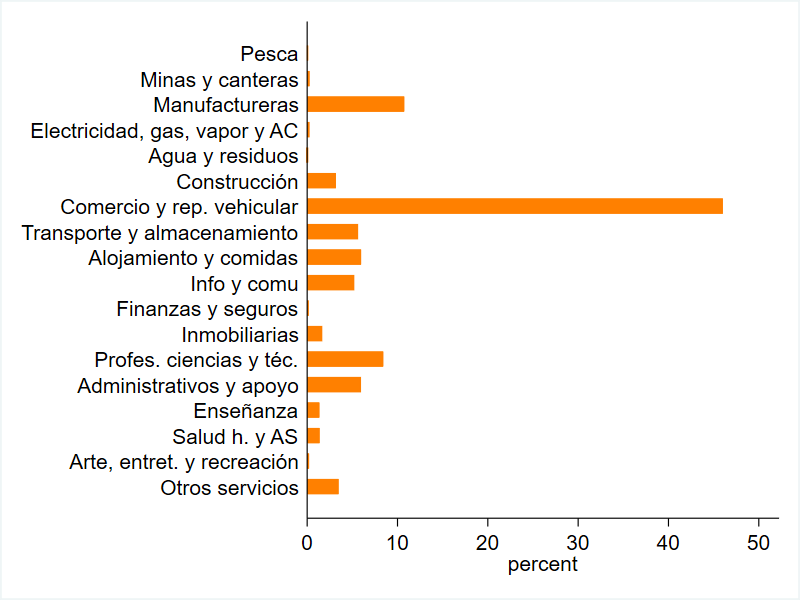
\includegraphics[scale = 0.5]{Figuras/Gráfico1_ciiu}
                \caption*{\it Nota: Elaboración propia}
                \label{fig: ciiu}
            \end{figure}
            %%% Figure 2
            \begin{figure}[H]
                \centering
                \caption{Estado de empresa como consecuencia del COVID-19 en el segundo trimestre del 2020.}
                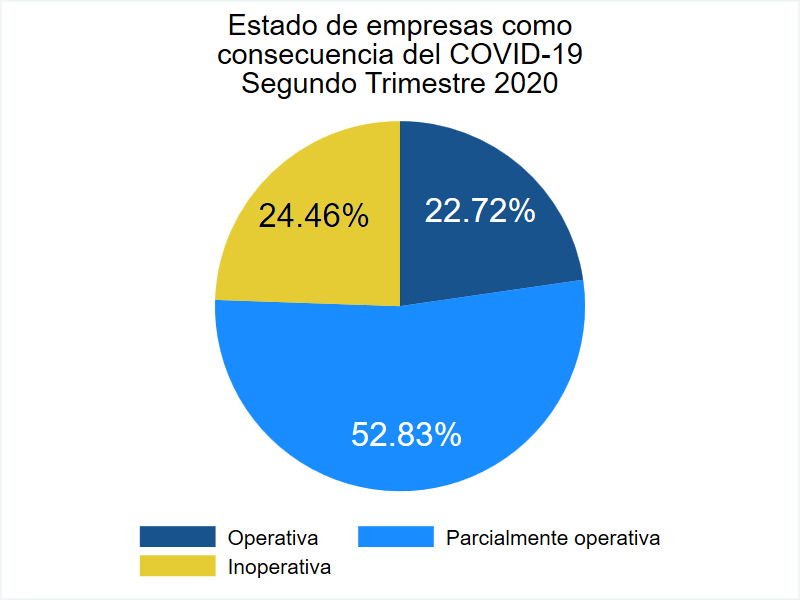
\includegraphics[scale = 0.5]{Figuras/Gráfico2_estado}
                \caption*{\it Nota: Elaboración propia}
                \label{fig: estado}
            \end{figure}
            %%% Figure 3
            \begin{figure}[H]
                \centering
                \caption{¿Considera que varió su venta como consecuencia del COVID-19?}
                \includegraphics[scale = 0.5]{Figuras/Gráfico3_varventas}
                \caption*{\it Nota: Elaboración propia}
                \label{fig: varventas}
            \end{figure}
            %%% Figure 4
            \begin{figure}[H]
                \centering
                \caption{Modalidad de trabajo asumida por la empresa en el segundo trimestre del 2020.}
                \includegraphics[scale = 0.5]{Figuras/Gráfico4_modtrabajo}
                \caption*{\it Nota: Elaboración propia}
                \label{fig: modtrabajo}
            \end{figure}
            %%% Figure 5
            \begin{figure}[H]
                \centering
                \caption{Principales problemas que enfrentaron por el COVID-19 en el 2020-2T.}
                \includegraphics[scale = 0.5]{Figuras/Gráfico5_problemas}
                \caption*{\it Nota: Elaboración propia}
                \label{fig: problemas}
            \end{figure}
            %%% Figure 6
            \begin{figure}[H]
                \centering
                \caption{Principales medidas que se tomaron con los trabajadores en el 2020-2T.}
                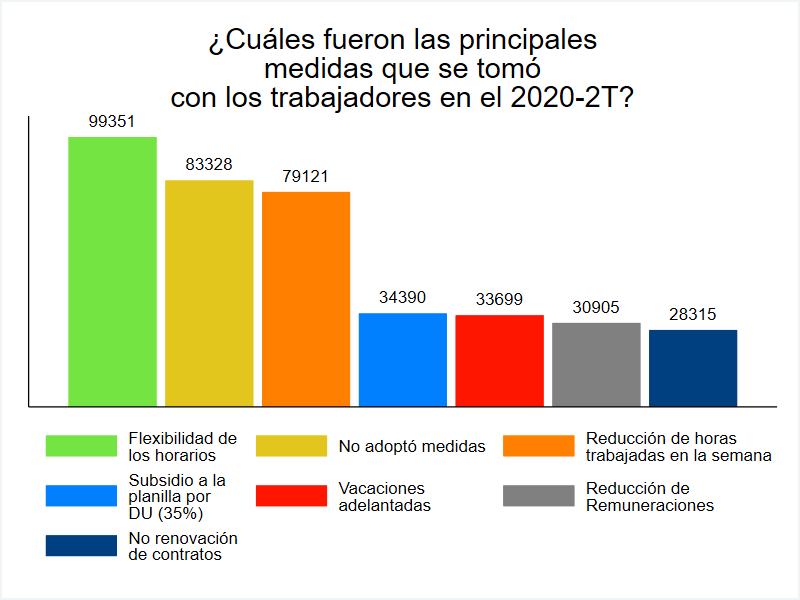
\includegraphics[scale = 0.5]{Figuras/Gráfico6_medidasL}
                \caption*{\it Nota: Elaboración propia}
                \label{fig: medidasL}
            \end{figure}
            %%% Figure 7
            \begin{figure}[H]
                \centering
                \caption{Los principales problemas financieros que presentó en el 2020-2T.}
                \includegraphics[scale = 0.5]{Figuras/Gráfico7_problemasf}
                \caption*{\it Nota: Elaboración propia}
                \label{fig: problemasf}
            \end{figure}
            %%% Figure 8
            \begin{figure}[H]
                \centering
                \caption{Acceso a programas de gobierno por actividad económica.}
                \includegraphics[scale = 0.5]{Figuras/Gráfico8_progragobiacce}
                \caption*{\it Nota: Elaboración propia}
                \label{fig: progragobiacce}
            \end{figure}
            %%% Figure 9
            \begin{figure}[H]
                \centering
                \caption{Programas del gobierno al que accedió.}
                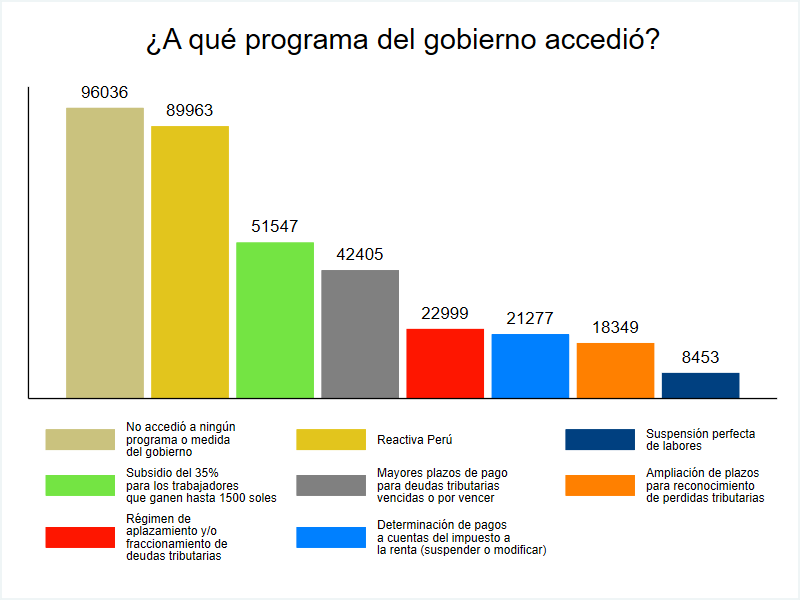
\includegraphics[scale = 0.5]{Figuras/Gráfico9_proggob}
                \caption*{\it Nota: Elaboración propia}
                \label{fig: proggob}
            \end{figure}
            %%% Figure 10
            \begin{figure}[H]
                \centering
                \caption{Motivos por los cuales dejaron de operar iniciada la pandemia.}
                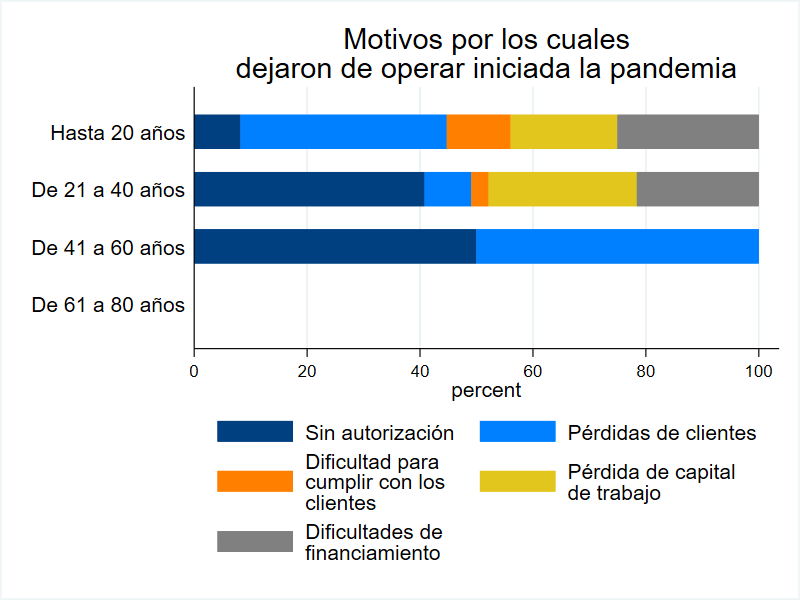
\includegraphics[scale = 0.5]{Figuras/Gráfico10_motinop}
                \caption*{\it Nota: Elaboración propia}
                \label{fig: motinop}
            \end{figure}
\end{document}